\documentclass[runningheads]{llncs}
%
\usepackage{graphicx}
\usepackage{float}
\usepackage{amssymb}
\usepackage{amsmath}
\usepackage{listings}
\usepackage{color}
\usepackage{xcolor}
\usepackage{booktabs}
\usepackage{tabularx}
\usepackage{cite}

\begin{document}
%
\title{Unbounding CBMC using Replication Reducing Abstraction}
%
%\titlerunning{Abbreviated paper title}
% If the paper title is too long for the running head, you can set
% an abbreviated paper title here
%
\author{Muralidhar Talupur\inst{1} 
  Lefan Zhang\inst{2} 
  Adrian Palacios\inst{1} 
  Mark R. Tuttle\inst{1}
  Mike Whalen\inst{1}
}
\authorrunning{Murali Talupur et al.}

%
\institute{Amazon/AWS/ARG \and
Univ of Chicago}

%
\maketitle              % typeset the header of the contribution
%
\begin{abstract}
Given a program CBMC first unwinds all the loops a small number of
times to obtain straight line code. In practice, these loops are
usually for traversing replicated data structures like arrays or lists
and in effect CBMC is able to prove programs correct only for small
data structures sizes. We describe a sound abstraction technique to
reduce replicated data structures to almost minimal sizes while
preserving all behaviors of interest. This in turn significantly
reduces the number loop iterations required to traverse them, letting
CBMC obtain fully unbounded proofs. This abstraction technique, called
Replication Reducing Abstraction or RRA, is inspired by similar
abstractions that have been successfully used in hardware and protocol
verification.

  
\keywords{CBMC  \and Abstraction \and Memory safety \and Security.}
\end{abstract}
%
%
%
\newcommand{\nop}[1]{}
\newcommand{\aid}{{\tt arr}}
\newcommand{\aabstid}{{\tt arr\$abst}}
\newcommand{\aobj}{arr}
\newcommand{\aabstobj}{\widehat{\aobj}}
\newcommand{\abst}{\alpha_{(c_1,c_2)}}
\newcommand{\abstm}{\alpha_{(c_1,c_2,...,c_m)}}
\newcommand{\conc}{\gamma_{(c_1,c_2)}}
\newcommand{\sizet}{{\tt uint}}
\newcommand{\tr}{\(Tr\)}
\newcommand{\trns}{Tr}
\newcommand{\trrd}{\(Tr_{read}\)}
\newcommand{\trnsrd}{Tr_{read}}
\newcommand{\trwr}{\(Tr_{write}\)}
\newcommand{\trnswr}{Tr_{write}}
\newcommand{\tras}{\(Tr_{assert}\)}
\newcommand{\trnsas}{Tr_{assert}}
\newcommand{\accns}{Acc}
\newcommand{\acc}{\(Acc\)}
\newcommand{\prog}{{\tt P}}
\newcommand{\progabst}{{\tt P\$abst}}
\newcommand{\aargid}{{\tt arr'}}
\newcommand{\arrayids}{\(ArraysAbst \)}
\newcommand{\indexids}{\(IndicesAbst \)}
\newcommand{\g}{{\bf G}}
\newcommand{\tp}{\mathcal{N}}
\newcommand{\chng}[3]{#1\{#2 \mapsto #3\}}
\newcommand{\ex}[4]{\langle #1, #2 \rangle \rightarrow \langle #3, #4\rangle}
\newcommand{\exstar}[4]{\langle #1, #2 \rangle \rightarrow^{*} \langle #3, #4\rangle}
\newcommand{\exa}[3]{\langle #1, #2 \rangle \rightarrow_{e} #3}
\newcommand{\exastar}[3]{\langle #1, #2 \rangle \rightarrow_{e}^{*} #3}
\newcommand{\rl}[2]{\frac{#1}{#2}}
\newcommand{\skp}{{\bf \tt skip}}
\newcommand{\fl}{{\bf \tt fail}}
\newcommand{\whld}[2]{{\tt while~#1~do~#2}}
\definecolor{commentgreen}{rgb}{0,0.6,0}
\definecolor{eclipseStrings}{RGB}{42,0.0,255}
\definecolor{eclipseKeywords}{RGB}{127,0,85}
\colorlet{numb}{magenta!60!black}

\lstdefinelanguage{json}{
    basicstyle=\normalfont\ttfamily,
    commentstyle=\color{eclipseStrings}, % style of comment
    stringstyle=\color{eclipseKeywords}, % style of strings
    showstringspaces=false,
    breaklines=true,
    string=[s]{"}{"},
    comment=[l]{:\ "},
    morecomment=[l]{:"},
    literate=
        *{0}{{{\color{numb}0}}}{1}
         {1}{{{\color{numb}1}}}{1}
         {2}{{{\color{numb}2}}}{1}
         {3}{{{\color{numb}3}}}{1}
         {4}{{{\color{numb}4}}}{1}
         {5}{{{\color{numb}5}}}{1}
         {6}{{{\color{numb}6}}}{1}
         {7}{{{\color{numb}7}}}{1}
         {8}{{{\color{numb}8}}}{1}
         {9}{{{\color{numb}9}}}{1}
}
\section{Introduction}


CBMC is being used by at AWS to verify memory safety and functional
correctness of foundational C libraries such as AWS C Common and AWS
Encryption SDK. It is a robust tool that can handle almost all of C
constructs seen in practice, and finds bugs that are very hard to find
by unit/integration testing. Moreover, CBMC is easy enough to deploy
that many developers use it routinely at AWS. But most of the current
proofs are bounded in the size of the inputs they can handle. For
instance, current proof of \emph{aws\_rray\_eq} program (shown below)
assumes a bound of size 20 on the input arrays.

\begin{figure}[H]
  \centering
  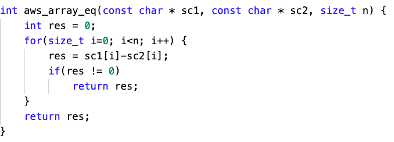
\includegraphics[scale=0.6]{Picture1.png}
  \caption{Arrays equals program}
\end{figure}

The reason is CBMC has to first unwind the ‘for’ loop a small number
of times, here 20, to obtain a straight-line code which can then be
translated into a SAT problem. Since the loop is used to traverse the
array, limiting the number of unwindings is in effect the same as
ignoring entries at indices greater than 20. For instance, the bug in
the following modified \emph{aws\_array\_eq} program will not be found by
unwinding the loop fewer than 100 times.

\begin{figure}[H]
  \centering
  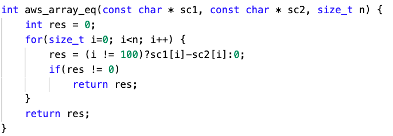
\includegraphics[scale=0.6]{Picture2.png}
  \caption{Buggy version}
\end{figure}

\nop{
We describe an abstraction technique that in conjunction with CBMC
allows us to write unbounded proofs of C programs with minimal user
effort. The key insight in our method is that by reducing replication in
the data structures in C programs we reduce the number of loop
unrollings required. Once this reduction is performed CBMC is then
able to give unbounded proofs for programs.}

This is an instance of a more general problem that is also seen in
hardware (HW) and protocol verification. HW designs have large
memories, register banks, buffers and such that exhibit a high degree
of replication. Data Type Reduction, studied by Long~\cite{long},
McMillan~\cite{mcmillan}, Wolpert~\cite{wolpert} and others, has been
successfully used to tackle this problem. The idea simply is that a
large, potentially unbounded data type can be replaced by a small
finite abstract data type that tracks specific values precisely and
the rest are replaced by abstract values. For example, a set of
indices [1..n] can be replaced by an abstract type [{\tt i},\(\bot\)]
which tracks a particular index {\tt i} precisely and the rest of the
indices imprecisely. This abstraction retains enough information to
decide value of terms like \({\tt i} \neq {\tt j}\) and {\tt a[i]}
precisely but not those of terms like \({\tt j} \neq {\tt k}\) and
{\tt a[k]} where {\tt j,k} are different from {\tt i}.

In case of distributed protocols like cache coherence protocols there
is replication in the form of multiple identical cache agents running
in different processes.  Replication reducing techniques such as the CMP
technique~\cite{self} have been used to scale model checkers to any
required bound size.

\nop{For example, in HW verification Data Type Reduction has been highly
successful. It is a special case of Abstraction Interpretation~\cite{abstint},
that has been studied by multiple works such as
Wolpert~\cite{wolpert}, Long~\cite{long}, McMillan~\cite{mcmillan} and
others. The idea simply is that a large, potentially unbounded data
type can be replaced by a small finite abstract data type that tracks
specific values precisely and the rest are replaced by abstract
values. For example, a set of indices [1..n] can be replaced by an
abstract type [{\tt i},\(\bot\)] which tracks a particular index {\tt i} precisely and
the rest of the indices imprecisely. This abstraction retains enough
information to decide value of terms like \({\tt i} \neq {\tt j}\) and {\tt a[i]} precisely but
not those of terms like \({\tt j} \neq {\tt k}\) and {\tt a[k]} where {\tt j,k} are different from {\tt i}.}

We can use a similar abstractions to reduce replication and help CBMC
scale to any required input size. Consider the \emph{aws\_array\_eq}
program again which compares two arrays by iterating over them. In
each iteration it compares {\tt sc1[i]} against {\tt sc2[i]} and
entries at different indices don’t interfere with one another. A bug
in this program will be localized to one particular index and what
happens at the other indices can be ignored.

If we can guess the precise location ‘c’ at which {\tt sc1} and {\tt
  sc2} differ we could have collapsed all the entries before ‘c’ into
one location and all the entries after ‘c’ into another
location. Reduced {\tt sc1} and {\tt sc2} arrays with just 3 indices
would still be sufficient to expose the bug in the program.

Because we don’t know the value of ‘c’ upfront, we introduce it as a
free variable and abstract the arrays {\tt sc1}, {\tt sc2} with
respect to it \emph{dynamically}. When we run CBMC it will try all
possible values for ‘c’ and for each value of ‘c’ the abstracted
arrays are of length only 3. If there is a bug in the original program
it will be found in the abstract program too. If the abstract program
has no bug then we can conclude that the original program is bug free
as well. Intuitively, the original program has a deep state space
whereas the abstract program has broad but shallow state space. CBMC
can completely explore the latter but not the former.

We call this abstraction Replication Reducing Abstraction or RRA for
short. We applied this technique to a collection of AWS C Common
examples that currently have bounded proofs using CBMC. These examples
are daunting enough that most of the tools in SVComp 2020 failed to
handle them in an unbounded fashion. We had to make slight
modification to the default {\tt memcpy} and {\tt memcmp} functions as
they use pointer arithmetic to traverse/access array contents. We
rewrote these to use clean array indexing instead as the current
version of RRA doesn't yet handle full pointer arithmetic.

We will next describe a minimal program model without pointer
arithmetic and use it to formally define how RRA transforms a
program. The section after that goes over the soundness of the
abstraction. Apart from soundness another concern when doing
abstraction is to eliminate or reduce spurious counterexamples. We
describe a simple transformation for properties that is quite
useful in reducing spurious failures. We end the paper by going over
the examples we have handled and surveying the related work.

%\section{RRA-Intuition}

The problem we see here is an instance of a more general problem that
is also seen in hardware (HW) and protocol verification. HW designs have large
memories, register banks, buffers that exhibit a high degree of
replication. In case of distributed protocols like cache coherence
protocols there is replication in the agents with multiple identical
cache agents running in different processes.  Replication reducing
techniques have been used successfully in HW~\cite{mcmillan} and
Protocol Verification~\cite{self} to scale Model Checkers to any
required bound size.

For example, in HW verification Data Type Reduction has been highly
successful. It is a special case of Abstraction Interpretation~\cite{abstint},
that has been studied by multiple works such as
Wolpert~\cite{wolpert}, Long~\cite{long}, McMillan~\cite{mcmillan} and
others. The idea simply is that a large, potentially unbounded data
type can be replaced by a small finite abstract data type that tracks
specific values precisely and the rest are replaced by abstract
values. For example, a set of indices [1..n] can be replaced by an
abstract type [{\tt i},\(\bot\)] which tracks a particular index {\tt i} precisely and
the rest of the indices imprecisely. This abstraction retains enough
information to decide value of terms like \({\tt i} \neq {\tt j}\) and {\tt a[i]} precisely but
not those of terms like \({\tt j} \neq {\tt k}\) and {\tt a[k]} where {\tt j,k} are different from {\tt i}.

RRA technique broadly belongs to the same class of
techniques. Consider \emph{aws\_array\_eq} program again which compares two
arrays by iterating over them. In each iteration it compares {\tt sc1[i]}
against {\tt sc2[i]} and entries at different indices don’t interfere with
one another. A bug in this program will be localized to one particular
index and what happens at the other indices can be ignored.

If we can guess the precise location ‘c’ at which {\tt sc1} and {\tt
  sc2} differ we could have collapsed all the entries before ‘c’ into
one location and all the entries after ‘c’ into another location. The
reduced {\tt sc1} and {\tt sc2} arrays with just 3 indices would still
be sufficient to expose the bug in the program.

Because we don’t know the value of ‘c’ upfront, we introduce it as a
free variable and abstract the arrays {\tt sc1}, {\tt sc2} with respect to
it. When we run CBMC it will try all possible values for ‘c’ and for
each value of ‘c’ the abstracted arrays are of length only 3. If there
is a bug in the original program it will be found in the abstract
program too. If the abstract program has no bug then we can conclude
that the original program is bug free as well. Intuitively, the
original program has a deep state space whereas the abstract program
has broad but shallow state space. CBMC can completely explore the
latter but not the former.

We next define the program model and RRA abstraction formally. In the
section after that we argue the soundness of this abstraction
technique.


\section{Program Model}~\label{sec:model}

\newcommand{\ra}{\(\rightarrow\)}
\newcommand{\wh}{{\tt while }}
\newcommand{\dt}{{\tt do }}

\subsection{Syntactic description}

CBMC compiles C programs into an intermediate form called
goto-programs with a limited number of instruction types. We use a
simplified model of goto-programs presented below to define RRA.

There are only three types of variables allowed in our program model:
{\tt bool}, {\tt uint} and {\tt array} over {\tt uint}. A program \prog{}
consists of global variable declarations followed by a series of
functions. Each function has a declaration followed by a list of
instructions.

More formally, the following grammar with the restrictions given after
it describes the allowed programs. We will use plurals to refer to a
list of things. For example, 'vars' refers to list of 'var'. In the
following {\tt V} and {\tt C} refer to set of all variable identifiers
and constants in the program. Entities in {\tt type writer} font refer
to terminals and those in normal font refer to non-terminals.

\begin{figure}[H]
  \centering
  \begin{tabular}{lcl}
    type & \ra & {\tt bool} \(|\) {\tt uint} \(|\) {\tt array[uint] of uint} \\
    program & \ra & decls funcs \\
    decl & \ra & type {\tt id}, {\tt id} \(\in\) {\tt V}   \\
    func & \ra & type id params instrs \\
    param & \ra & decl \\
    &&\\
    instr & \ra & \wh exp {\tt do} instrs (while-do) \\
    & \ra & exp {\tt =} exp (assign) \\
    & \ra & {\tt assert} exp (assert) \\
    & \ra & {\tt assume} exp (assume) \\
    & \ra & {\tt return} exp (return) \\
    & & \\
    exp & \ra & {\tt id} where {\tt id} \(\in {\tt V} \cup {\tt C}\) \\
    & \ra & {\tt a[} exp {\tt ]} \\
    & \ra & exp {\tt +} exp \\
    & \ra & exp {\tt rel\_op} exp, where {\tt rel\_op} \(\in \{==, \neq\}\) \\
    & \ra & exp{\tt ?}exp{\tt :}exp \\
    & \ra & {\tt funcname} exp
    
  \end{tabular}
\end{figure}

 
We have allowed only one type of arithmetic expression and two types
of relational expressions to keep the presentation
simple. Generalizing to other types of expressions is
straightforward. Note that the whole system is closed, there are no
inputs read from outside. A program taken together with it's CBMC
proof harness is a closed system, so this is not a limitation. We
don’t allow functions to have local variables. We further make the
following restrictions to simplify the presentation:

\begin{itemize}



\item[{\bf A1}]  Variables are initialized before being used for the first time.

\item[{\bf A2}] We assume there is a {\tt main} function that serves
  as the entry point.

\item[{\bf A3}] All functions have only one argument, except {\tt
  main} which has none.

\item[{\bf A4}] Every function apart from {\tt main}
  has a return value.
\end{itemize}


Note that we have not considered explicit use of pointers in this
language. \emph{We assume all memory accesses are through array
references.} Extension to the general model with pointers will be
considered in future work.

The model described here corresponds to a program under verification
along with its proof harness, which supplies all the inputs and
\emph{closes} the system. But in a proof harness inputs are allowed to
take all possible values (subject to any \emph{assumptions}) whereas
in the model we force inputs to take a specific value. Our objective
here is to show that every trace of the concrete program has a
corresponding abstract trace. There is no loss of generality because
our main soundness theorem holds no matter what specific inputs are
chosen.

\subsection{Semantics}

With each function {\tt foo} we will associate a ghost
variable~\footnote{A variable that monitors but doesn't in any way
  affect the program execution.} \(ret_{\tt foo}\) that holds the
return value of {\tt foo} after each invocation of {\tt foo}.\nop{ To
define program semantics we assume we have call stack {\tt stack} that
holds the real parameters passed to functions and a variable {\tt
  stacktop} that has exact value at the top of {\tt stack}.} A state
\(s\) of program {\tt P} is then given by
\begin{itemize}

\item valuation of all variables in {\tt V}
\item valuation of the ghost variables.
  
\end{itemize}

Denote by \(s({\tt v})\) the value of variable {\tt v} from {\tt V} in
state \(s\).  In the initial state \(Init\) all variables are
initialized to a special value \(\tp\), which stands for
nondeterministic value. A read from \(\tp\) can return any value from
the type of the variable to which it is assigned. Multiple reads from
a variable with value \(\tp\) can return different values even if the
variable has not been assigned in the interim.

We write \(\chng{s}{\tt x}{\tt v}\) to denote the state derived from \(s\) by changing
value of variable {\tt x} to \(v\). We give the small-step semantics for the program below.

\subsubsection{Semantic rules for expressions}
First define
\(\rightarrow_e\) that gives semantic meaning to expressions. We will
write \(\exastar{{\tt exp}}{s}{i}\) to mean expression {\tt exp} reduces
to constant \(i\) in state \(s\) by repeated application of semantic
rules. 

For a variable {\tt v} in {\tt V}, we have the following rule:

\[\rl{}{\exa{{\tt v}}{s}{s({\tt v})}}\]

For array index expression:


\[\rl{\exastar{{\tt exp}}{s}{i}}{\exa{{\tt a[exp]}}{s}{{\tt a[}i{\tt ]}}}\]


For arithmetic expression:

\[\rl{{\exastar{{\tt exp1}}{s}{i1}}, {\exastar{{\tt exp2}}{s}{i2}}}{\exa{{\tt exp1 + exp2}}{s}{{i1 + i2}}}\]

For relational expression:

\[\rl{{\exastar{{\tt exp1}}{s}{i1}}, {\exastar{{\tt exp2}}{s}{i2}}}{\exa{{\tt exp1 ~rel\_op ~exp2}}{s}{{i1 ~rel\_op ~i2}}}\]

where {\tt rel\_op} determines the semantic \(rel\_op\) used in the rule.

For if-then-else expression:

\[\rl{{\exastar{{\tt exp}}{s}{b}}, {\exastar{{\tt exp1}}{s}{i1}}, {\exastar{{\tt exp2}}{s}{i2}} }{\exa{{\tt exp ? exp1 : exp2 }}{s}{b?i1:i2}}\]

As semantics for function call expression requires semantics for
instructions we will defer it to the next section.

\subsubsection{Semantic rules of instructions}

We write \(\ex{c}{s}{\skp}{s'}\) to mean that executing instruction
\(c\) starting at state \(s\) leads to state \(s'\). Essentially,
\(\skp\) denotes an empty instruction. An empty list of instructions
can also be represented by a single \(\skp\) instruction.

A list of instructions will be treated as a sequence of instructions
separated by a semi-colon ({\tt ;}). First we have the following rule
for sequencing of instructions:

\[\rl{\ex{c_0}{s}{c'_0}{s'}}{\ex{c_0;c_1}{s}{c'_0;c_1}{s'}}\]

For \(\skp\) instruction we have

\[\rl{}{\ex{\skp;c_1}{s}{c_1}{s}}\]

\nop{
An empty list of instructions is treated
as a \(\skp\) instruction. That is,

\[\rl{}{\ex{[]}{s}{\skp}{s}}\]}


We also have \(\fl\) instruction to capture program failure with the following semantic rule

\[\rl{}{\ex{\fl;c}{s}{\fl}{s}}\]

Execution of a well formed program always ends with either with \(\skp\) or \(\fl\)
instruction.
\nop{
For handling assigments with function expression, assume we
have the following variables and functions
\begin{itemize}

\item {\tt pop()} that pops the top element of {\tt stack}, modifies
  {\tt stacktop} and returns the modified stack
\item \({\tt push(v)}\) that pushes value \({\tt v}\) on top of
  {\tt stack}, modifies {\tt stacktop} and returns the updated stack.
\end{itemize}
}



For the {\tt while-do} instruction we have the following two rules

\[\rl{\exastar{{\tt cond}}{s}{true}} {\ex{\whld{cond}{body}} {s} {{\tt body;}\whld{cond}{body}}{s}}\]

and

\[\rl{\exastar{{\tt cond}}{s}{false}} {\ex{\whld{cond}{body}} {s} {\skp} {s}}\]


For assigns:

\[\rl{\exastar{e2}{s}{ v}}{\ex{\tt e1 = e2} {s} {\skp} {\chng{s} {e1} {v}}}\]


For assert instructions:

\[\rl{\exastar{{\tt e}}{s}{true} }{\ex{{\tt assert(e)}} {s} {\skp} {s}}\]

and

\[\rl{\exastar{{\tt e}}{s}{false}}{\ex{{\tt assert(e)}} {s} {\fl} {s}}\]

For assume instructions:

\[\rl{\exastar{{\tt e}}{s}{true}}{\ex{{\tt assume(e)}} {s} {\skp} {s}}\]

and

\[\rl{\exastar{{\tt e}}{s}{false}}{\ex{{\tt assume(e)}} {s} {\fl} {s}}\]
  
For return instructions:


\[\rl{\exastar{{\tt e}}{s}{{ v}} }{\ex{{\tt return(e)}} {s} {\skp} {\chng{s}{{\tt ret_{foo}}}{v}} }\]

We can now define the semantic rule for function call expression. In
the following, \({\tt body_{foo}}\) denotes the list of instructions
following declaration of {\tt foo(arg)}. And similar to
\(\rightarrow_{e}^{*}\), we use \(\rightarrow^{*}\) to denote repeated
application of the single step semantic rule \(\rightarrow\). \nop{We have the
  following rules for function call statement:

\[\rl{\exa{{\tt arg}}{s}{{ v}} }{\ex{\tt foo(arg)}{s}{{{\tt arg = }} v;{\tt body_{foo}}}{s}}\]

and

\[\rl{}{\ex{\tt x = foo(exp)}{s}{\tt foo(arg);x=ret_{\tt foo}}{s}}\]
}


\[\rl{{\exastar{{\tt arg}}{s}{{ v}}}, {\exstar{{\tt arg} = v; {\tt body_{foo}}}{s}{\skp}{s'}} }{\exa{{\tt foo(arg)}}{s}{{s'({\tt ret_{foo}})}}}\]

As the semantic rule makes it clear function arguments are passed by
value.

Given a program {\tt P} that has an entry point function {\tt main()}
a {\bf rule trace} is a sequence of configurations, related by either
\(\rightarrow\) or \(\rightarrow_e\), starting at \(\langle{\tt
  body_{main}}, Init \rangle\) and ending in a configuration \(\langle
last, s_n\rangle\) where \(last \in \{\skp, \fl\}\). An {\bf
  instruction trace} is obtained by projecting out configurations that
are related to the preceeding configuration by \(\rightarrow_e\). An
{\bf execution trace} is projection of each configuration in an
instruction trace on to the state component of it. Essentially, an
execution trace just keeps next states from executing
instructions. Evaluation of expressions don't contribute to the trace.

\nop{
\begin{definition}[Execution Trace]

  An execution trace \(t\) of program {\tt P} is a sequence of states
\(s_0 = Init, s_1,s_2,…s_n\) such that starting at \(\langle {\tt
  main}, s_0 \rangle\) repeated application of execution rules above
lead us to \(\langle \skp, s_n\rangle\) or  \(\langle \fl, s_n\rangle\).

\end{definition}
}

\nop{
From now on, for syntactic entities such as the program {\tt P} will
use typewriter font and semantic entities like the state \(s\) using
math-mode. Entities which play both a semantic and syntactic role like
\(\abst\) and \arrayids{} will be given in math-mode.
}

\section{Formalizing RRA}~\label{sec:rra}

User first specifies the arrays to be abstracted along with the shapes
to use. In \emph{aws\_array\_eq} example the shape used can be written
as {\it *c*}, that is, track one location precisely and abstract the
locations before and after it. For the rest of this presentation, we
will fix the shape to be {\it *c*c*} which keeps track of two locations
\(c_1 < c_2\). In general, the shape  {\it *c*c*} can also represent
cases where \((c_1 = c_2 - 1)\), that is, they are adjacent. This
would complicate \(\abst\) and \(\conc\) functions described
below. To keep the presentation simple we assume \(c_1 < c_2 -
1\). Let the array to be abstracted be \aid. Extension to other
shapes and multiple arrays is straightforward. The abstraction
function \(\abst\) mapping concrete indices to abstract indices is
parameterized by the values \(c_1, c_2\) for the precise locations and
is as follows:

\begin{figure}[H]
  \centering
  \begin{tabular}{ccl}
    \(\abst(v)\) & = & 0 if \(v < c_1\) \\
    &=& 1 if \(v = c_1\) \\
    &=& 2 if \(c_1 < v < c_2\) \\
    &=& 3 if \(v = c_2\) \\
    &=& 4 if \(v > c_2\)
    \end{tabular}
\end{figure}

There will be a corresponding concretization function as follows:

\begin{figure}[H]
  \centering
  \begin{tabular}{ccl}
    \(\conc(0)\)  &=& \(\{v \mid \mbox{ where } 0 \leq  v < c_1\}\) \\
    \(\conc(1)\)  &=& \(\{c_1\}\) \\
     \(\conc(2)\) &=& \(\{v \mid \mbox{ where } 0 \leq  c_1 < v < c_2\}\) \\ 
    \(\conc(3)\)  &=& \(\{c_2\}\) \\
     \(\conc(4)\) &=& \(\{v \mid \mbox{ where } 0 \leq  v > c_2\}\)
    \end{tabular}
\end{figure}

Misusing notation slightly \(\abst\) and \(\conc\) can be applied to arrays too.
Let length of \(\aobj\) be \(l\) such that \(c_2 < l\) and its range be \sizet. Then

\(\abst(\aobj)\) is an array \(\aabstobj\) of length 5 such that

\begin{figure}[H]
  \centering
  \begin{tabular}{ccl}
    \(\aabstobj[1]\)  &=& \(\aobj[c_1]\) \\
    \(\aabstobj[3]\)  &=& \(\aobj[c_2]\) \\
    \(\aabstobj[x]\)  &=& \(\tp\) for \(x \notin [1,3]\)\\
    \end{tabular}
\end{figure}

The special value \(\tp\) at abstract locations in \(\aabstobj\) indicates that
reads from those locations can return any value.

\begin{remark}
Abstraction function \(\abst\) assumes that \(\aobj\) is at least
\(c_2+1\) elements in length. Now the lowest value for \(c_2\) can be
\(2\) which happens when \(c_1 = 0\). So \(\aobj\) has to be of length
at least 3 and soundness results discussed below hold only for arrays
of size 3 or more. Regular CBMC without abstraction is any way
adequate for smaller arrays and abstraction is meant to make large
arrays manageable.
\end{remark}

Given an
array \(\aabstobj\) of length 5, \(\conc(\aabstobj)\) is the set of
all arrays \(\aobj\) of length at least \(c_2+1\) such that

\begin{figure}[H]
  \centering
  \begin{tabular}{ccl}
    \(\aobj[c_1]\)  &=& \(\aabstobj[1]\) \\
    \(\aobj[c_2]\)  &=& \(\aabstobj[3]\) \\
    \(\aobj[x]\)  &=& \(v \in \sizet\) for \(x \notin [c_1,c_2]\)\\
    \end{tabular}
\end{figure}

Note that an abstract array can concretize to a set of different
concrete arrays. Abstracting and then concretizing an array will give us a
set containing the original array. That is,
\[\aobj \in \conc(\abst(\aobj))\]

Functions \(\abst\) and \(\conc\) operate on states and since states are
available only during execution these two functions are used
dynamically as the program is being model checked.

We will next define a function \tr{} that syntactically transforms a
given program \prog{} to a program \progabst. This will essentially involve
identifying entities to be abstracted, substituting them with abstract
entities, and rewriting program logic to work with abstracted
entities.

\subsection{Preprocessing phase}

In the abstract program \aid{} will be replaced by \aabstid{}. Now
\aabstid{} might be passed to other functions as an argument, say as
an argument named \aargid{} for some function {\tt foo}. When we
transform \prog{} we have to change \aargid{} to an abstract entity as
well. We first identify all arrays in all functions that can get their
value from \aid{}, the main array being abstracted. This can be done
statically by following assignments in function bodies, tracing
arguments as they are passed between functions and computing a closure
of the possible set of values for each array identifier. If an
identifier \aargid{} can get value from the array to be abstracted
and also from a normal array then our abstraction procedure throws an
exception. That's because we have to rewrite {\tt foo} to handle the case
when its argument is an abstract array but we also need to keep it as
is for the case when it receives a normal array argument. Assuming
this doesn’t happen we identify the set \arrayids{} of array
identifiers that need to be abstracted.

\begin{remark}
Requiring that an array identifier not get values from abstract and normal
arrays is quite restrictive. But as we are relying on array
names to keep track of heap objects we necessarily introduce
imprecision in our method. For a general method we should
determine if an array is abstract or not using its address, not its
name.
\end{remark}

Any variable used to iterate over abstract arrays also needs to be
replaced with a new variable with reduced range. This is what will
allow us to shorten the traces CBMC has to explore. An
intra-procedural closure analysis is performed starting with the set
\(I_0\) of expressions that directly index into the arrays in
\arrayids. For each expression we also add it's sub-expressions to the
set. Any expression (along with it's sub-expressions) that is assigned
to an expression in \(I_0\) is added to the set \(I_1\) (which is
initialized to \(I_0\)) and so on till we reach a fix point. Now we
intersect this with the set of variables appearing in the conditions
of while loops. Any variable appearing in both sets is added to the
set \indexids.

For example, consider the following program.

\begin{figure}[H]
  \centering
  \begin{tabular}{l}
    {\tt i = 0;} \\
    {\tt res = true;} \\
    {\tt while( i $!=$ len) do \{}  \\
    \hspace{1cm} {\tt j = i;} \\
    \hspace{1cm} {\tt res = res \&\& (arr[j] $!=$ 10);} \\
    \hspace{1cm}  {\tt i = i + 1;} \\
    \}\\
    \end{tabular}
\end{figure}
      
\(I_0\) = \{{\tt j}\}, \(I_1 =\) \{{\tt i, i+1, j}\}. Since only i appears in the condition of the while loop \indexids = \{i\}.

As another example consider the following program where only {\tt arr} is being abstracted:

\begin{figure}[H]
  \centering
  \begin{tabular}{l}
    {\tt i = 0;} \\
    {\tt res = true;} \\
    {\tt while( i $!=$ len) do \{}  \\
    \hspace{1cm} {\tt j = i;} \\
    \hspace{1cm} {\tt res = res \&\& (arr[arr1[j]] $!=$ 10);} \\
    \hspace{1cm}  {\tt i = i + 1;} \\
    \}\\
    \end{tabular}
\end{figure}

Here \(I_0\) = \{{\tt arr1[j], j}\}, \(I_1\) = \{{\tt i, j, arr1[j]}\} and \indexids = \{{\tt i}\}.



\subsection{Program Transformation}

    
Using \arrayids{} and \indexids{} computed in the preprocessing phase, we
will describe the program transformation \tr{} that rewrites concrete
program into an abstract program. The transformation first adds the
declaration
\begin{figure}[H]
  \centering
      {\tt uint c1, c2;}
\end{figure}

to represent the free reference variables used in the
abstraction. For all  in \({\tt var} \in\) \indexids{} we add the declaration

\begin{figure}[H]
  \centering
      {\tt type var\$abst}
\end{figure}

where {\tt type} matches the type of {\tt var} in case of
\indexids. In case of \({\tt arr} \in\) \arrayids{} it adds 

\begin{figure}[H]
  \centering
      {\tt array[5] of uint arr\$abst}
\end{figure}

That is, we declare a new array variable {\tt arr\$abst} with exactly
5 cells. The number 5 is determined by the shape \(*c*c*\) we are
using for the abstraction.

Next \tr{} rewrites each function as follows.

\subsubsection{Rewrites for function declarations}

Every function has a declaration followed by a list of
instructions. Function declarations are left unchanged:

\begin{figure}[H]
  \centering
  \begin{tabular}{lcl}
    \tr({\tt type funcname(var)}) & \ra & {\tt type funcname( var)}
  \end{tabular}
\end{figure}

If \({\tt var} \in\)
\indexids{} \(\cup\) \arrayids{} we add the following assignment right after the
declaration

\begin{figure}[H]
  \centering
      {\tt var\$abst} = \(\abst({\tt var})\)
\end{figure}

\begin{remark}
As the subsequent rewrite rules show we make sure a function always
returns a concrete value. The burden of abstracting the
return value is placed on the instruction containing the function
call.
  
\end{remark}

\subsubsection{Rewrite for instructions}

For rewriting instructions, \tr{} will make use of two helper function
\trrd, \trwr{} both of which operate on expressions.

\begin{figure}[H]
  \centering
  \begin{tabular}{lcl}
    
\tr({\tt while cond do instrs}) & \ra & {\tt while(}\trrd{\tt (cond)) do} \tr{\tt (instrs)} \\

\tr({\tt exp1 = exp2}) & \ra &  if {\tt exp1} \(\in\) \indexids{} then \\
&&                                          {\tt exp1\$abst  =} \(\abst\)(\trrd({\tt exp2})) \\
      &&                                    else \trwr({\tt exp1}) {\tt =} \trrd({\tt exp2}) \\

\tr({\tt funcname(exps)})  & \ra &   {\tt funcname(}\trrd({\tt exps}){\tt )} \\

\tr({\tt assert(exp)})  & \ra &  {\tt assert(}\trrd ({\tt exp}){\tt )} \\

\tr({\tt assume(exp)})  & \ra & {\tt assume(}\trrd ({\tt exp}){\tt )} \\
 
\tr({\tt return(exp)}) & \ra &  {\tt return(}\trrd ({\tt exp}){\tt )} \\ 
                                       
  \end{tabular}
\end{figure}


\subsubsection{Rewrite for expressions}

Expressions are transformed using \trrd{} and \trwr. We assume the
availability of a function {\tt nondet()} that returns a random value
from {\tt uint}. We first define \trrd.

\begin{figure}[H]
  \centering
  \begin{tabular}{lcl}
    
\trrd ({\tt i}) & \ra & if {\tt i} \(\in\) \indexids{} then  \(\conc\){\tt (i\$abst)} else {\tt i} \\

\trrd ({\tt a[exp]}) & \ra & if {\tt a} \(\in\) \arrayids{} then \\
		&&	 \hspace{0.5cm} {\tt is\_precise(exp’)? a\$abst[exp’] : nondet()} \\
&&	 \hspace{0.5cm}  where {\tt exp’ = }\(\abst\) (\trrd ({\tt exp})) \\
%%&& \hspace{0.5cm} {\tt nondet} is a value from {\tt a's} range \\
		  &&     else {\tt a[}\trrd {\tt (exp)]} \\

\trrd ({\tt exp1 + exp2}) & \ra & \trrd ({\tt exp1}) {\tt +} \trrd ({\tt exp2}) \\

\trrd ({\tt exp1 rel\_op exp2}) & \ra &  \trrd ({\tt exp1}) {\tt rel\_op} \trrd ({\tt exp2}) \\

\trrd ({\tt exp~?~exp1~:~exp2}) & \ra &  \trrd ({\tt exp}) {\tt ?} \trrd ({\tt exp1}) {\tt :} \trrd ({\tt exp2}) \\

\trrd ({\tt funcname(exps)}) & \ra & {\tt funcname}(\trrd ({\tt exps})) \\

  \end{tabular}
\end{figure}

Function {\tt is\_precise} used above is defined as follows:

{\tt is\_precise(v) = v}\(\in\){\tt \{1,3\}? true : false}

Recall that we are abstracting using \(*c*c*\) and so indices 1, 3 are
the precise locations. Observe that \trrd{} always returns a concrete
value, never an abstract value. In case it is applied to an abstracted
index {\tt i\$abst}, it concretizes it as \(\conc\)({\tt i\$abst}),
allowing for a set of values all of which are concrete. This is a
slight abuse of notation as we are replacing a variable {\tt i} by a
set. The intended meaning is we can non-deterministically pick any
value from the set.
 
Next \trwr{} which is used to rewrite left hand sides of assign
instructions is defined.

\begin{figure}[H]
  \centering
  \begin{tabular}{lcl}

    \trwr({\tt i}) & \ra & if {\tt i} \(\in\) \indexids{} then {\tt i\$abst} else {\tt i} \\

\trwr({\tt a[exp]}) & \ra & if {\tt a} \(\in\) \arrayids{} then {\tt a\$abst[}\(\abst\))(\trrd ({\tt exp}){\tt]} \\
	               &&     else {\tt a[}\trrd({\tt exp}){\tt ]} \\

\trwr({\tt exp1 rel\_op exp2}) & \ra & throw exception (cannot occur on lhs) \\

\trwr({\tt exp1 + exp2}) & \ra & throw exception (cannot occur on lhs) \\

\trwr({\tt exp~?~exp1~:~exp2}) & \ra & throw exception (cannot occur on lhs) \\

\trwr({\tt funcname(exps)}) & \ra & throw exception (func exp cannot be on the lhs) \\

   \end{tabular}
\end{figure}





Like {\tt P} the abstracted program {\tt P\$abst} too has states comprising of
valuations of variables. The only
difference is that states of {\tt P\$abst} have abstracted values for
entities corresponding to \arrayids{} and \indexids. Everything else is
the same. In particular, the initial state \(Init\) of {\tt P} matches the
initial state  \(Init\$abst\) of {\tt P\$abst}, except for entities
in \arrayids{} and \indexids{} which appear abstracted in \({Init\$abst}\).

\section{ Proof of soundness}

Given a program \prog{} and assertion {\tt assert(exp)} we want to
establish that if the abstracted assertion {\tt assert(\trrd(exp))}
holds in the abstract program \progabst{} then {\tt assert(exp)} holds
in \prog. Recall that we are using the shape \(*c*c*\) and by
definition of \(\abst\) and \(\conc\) functions the arrays being
abstracted using \(*c*c*\) shape must have lengths greater than 3. All
the results below implicitly assume this.

In Lemma 2 we prove that any transition from a state \(s_1\)
to another state \(s_2\) using an instruction {\tt inst} is matched in
\progabst{} by a transition between \(\hat{s}_1\) to \(\hat{s}_2\),
where \(\hat{s}_i\) is an abstraction of state \(s_i\), made precise
in the definition below, using the instruction \(\trns({\tt
  inst})\). We also establish that \(\hat{s}_i\) is an
over-approximation of \(s_i\) as made precise by Lemma 1. Together
Lemma 1 and Lemma 2 imply that any offending trace in \prog{} will
have a counter part in \progabst{}. Conversely, if there are no
offending traces in \progabst{} there are none in \prog{} either. That
is, there exists a \emph{simulation} relation between \prog{} and
\progabst with traces of former contained in those of the latter. So
proving via model checking that \progabst{} is correct with respect to
asserts of interest is enough to guarantee that the same asserts hold in
\prog{} as well.

First, we
generalize the abstraction operation \(\abst\) to work on the entire
state. A state \(s\) of \prog{} is map from variables to their values.

\begin{definition}
Given a state \(s\) of program {\tt P} it's abstraction, denoted by
\(\abst(s)\), is obtained by replacing every {\tt id} in \arrayids{}
\(\cup\) \indexids{} by {\tt id\$abst} and abstracting the value \(s({\tt
  id})\) by \(\abst\). All other variables and values are left
unchanged.
\end{definition}



We have the following lemma relating \(s\) and \(\abst(s)\) given an
expression {\tt exp} of {\tt P}.

\begin{lemma}

The value of {\tt exp} in state \(s\) is contained in the set of
possible values for \(\trnsrd({\tt exp})\) in abstract state
\(\abst(s)\). Denoting \(\abst(s)\) by \(\hat{s}\) we have \[s({\tt exp}) \in \hat{s}(\trnsrd({\tt exp}))\]
  
\end{lemma}

\begin{proof}

We can prove this by case splitting on {\tt exp}. We will show it
for couple of cases as other cases are similar.

 Consider the case {\tt exp} is {\tt i} where \({\tt i} \in\)
 \indexids. In {\tt P\$abst}, it will be replaced by {\tt i\$abst} and
 \(\trnsrd(exp)\) will be \(\conc({\tt i\$abst})\). By definition of
 concretization function the set of concrete values includes the
 original value. So we have \(s({\tt exp}) \in \hat{s}(\trnsrd({\tt exp}))\).

 As another case let {\tt exp} be {\tt a[i]} where \({\tt a} \in\)
 \arrayids{} and \({\tt i} \in\) \indexids. Then \[\trnsrd({\tt
   a[i]})\] is {\tt is\_precise(i’)? a\$abst[i’] : nondet} where {\tt
   i’ = }\(\abst\) (\trrd ({\tt i})). If {\tt is\_precise(i’)} holds
 then we get back the value stored at {\tt a[i]}, and the lemma
 holds. Otherwise, we get {\tt nondet}, that is any possible value
 from range of {\tt a}. In this case too the lemma holds.

 Other cases are proved similarly.
 
 \qed
  
\end{proof}

\nop{Conversely, given an abstract state \(s’\) corresponding concrete
  states are obtained by applying \(\conc\) to abstract version of
  each array in \arrayids and abstract version of each variable in
  \indexids.  For each abstract entity, the concrete set will have
  multiple values and we pick some value from each set
  non-deterministically and independently. Note that \( s \in
  \conc(\abst(s))\).}


Before we prove the theorem, recall that when \tr{} is applied to {\tt
  P}, it adds new declarations at the beginning of {\tt P} and new
assignments at beginning of functions if their arguments are in
\indexids{} \(\cup\) \arrayids. Other than that it doesn’t add any new
instructions and doesn’t remove any existing
instructions. Syntactic structure of {\tt P} and {\tt
  P\$abst} are quite similar. Semantically, we have the following
lemma relating {\tt P} and {\tt P\$abst}.

\begin{lemma}
  Given an execution trace \(Init, s_1,....s_n\) of {\tt P}, for each
  transition \(s_{i-1}\) \(\rightarrow s_{i}\) either
  \(\abst(s_{i-1})\) \(\rightarrow \abst(s_{i})\) is a valid transition in {\tt
    P\$abst} or there exists sequence of intermediate states \(int_{1}, int_{2}..\) such that \(\abst(s_{i-1})\)
  \(\rightarrow int_{1} \rightarrow int_{2} ...\) \(\rightarrow \abst(s_i)\) is a valid
  sequence of transitions in {\tt P\$abst}.
\end{lemma}

\begin{proof}

 Assume the statement holds for prefix \(Init, s_1, ...,
 s_{i-1}\). For the base case \(Init\$abst = \abst(Init)\) is the
 initial state of {\tt P\$abst} by construction.

 We will prove the inductive step by matching the transition from
 \(s_{i-1}\) to \(s_i\) in {\tt P\$abst}. Since there are too many
 sub-cases we will consider only two representative cases here.

 Consider the case where the concrete transition is due to an
 assignment {\tt e1 = e2} where {\tt e1} is in {\tt V}  but not in \indexids. So
 \(s_{i-1}\) and \(s_i\) are related by the rule for assignment
 statements:

\[\rl{\exastar{e2}{s_{i-1}}{\tt v}}{\ex{\tt e1 = e2} {s_{i-1}} {\skp} {\chng{s_{i-1}} {e1} {v}}}\]

with \(s_i\) equal to \({\chng{s_{i-1}} {e1} {v}}\).

The corresponding statement in {\tt P\$abst} is {\tt \trwr({\tt e1}) =
  \trrd({\tt e2})} which would reduce to {\tt e1} = \trrd({\tt
  e2}). At state \(\abst(s_{i-1})\) the following rule will apply

\[\rl{\exastar{\tt \trnsrd(e2)}{\abst(s_{i-1})}{\tt v'}} {\ex{\tt e1 = \trnsrd(e2)} {\abst(s_{i-1})} {\skp} {\chng{\abst(s_{i-1})} {e1} {v'}}}\]

By previous lemma, the set of values of \trrd({\tt e2}) in
\(\abst(s_{i-1})\) contains {\tt v} the value of {\tt e2} in state
\(s_{i-1}\). So we can have {\tt v' = v} in the above rule. That is, at \(\abst(s_{i-1})\) this rule applies

\[\rl{\exastar{\tt \trnsrd(e2)}{\abst(s_{i-1})}{\tt v}} {\ex{\tt e1 = e2} {\abst(s_{i-1})} {\skp} {\chng{\abst(s_{i-1})} {e1} {v}}}\]

Since {\tt e1} is in {\tt V} but not in \indexids{} it is retained as is in the
abstract program {\tt P\$abst}. This means \({\tt \chng{\abst(s_{i-1})}
  {e1} {v}}\) is equal to \(\abst({\tt s_i})\) proving the inductive step in this case.

As another case, suppose {\tt e1} was in \indexids. Then the
assignment statement in {\tt P\$abst} would be {\tt {e1\$abst} =
  \(\abst(\)\trrd({\tt e2})\()\)}.

At abstract state \(\abst(s_{i-1})\) expression \(\abst(\)\trrd({\tt
  e2})\()\) can evaluate to \(\abst(v)\) where \(v\) is the value of
{\tt e2} in \(s_{i-1}\) (again by the previous lemma). So at \(\abst(s_{i-1})\) the following rule will apply

\[\rl{\exastar{\tt \trnsrd(e2)}{\abst(s_{i-1})}{\abst({\tt v})}}
     {\ex{\tt e1\$abst = \abst(\trnsrd(e2))} {\abst(s_{i-1})} {\skp} {\chng{\abst(s_{i-1})} {\tt e1\$abst} {\abst({\tt v})}}}\]

By construction \(\chng{\abst(s_{i-1})} {\tt e1\$abst} {\abst({\tt
    v})}\) is equal to \(\abst(s_i)\). Note that the evaluation
\({\exastar{\tt \trnsrd(e2)}{\abst(s_{i-1})}{\abst({\tt v})}}\)
involves function calls in \(\trnsrd\) and will introduce some
intermediate states \(int_1, int_2...\) as allowed by the statement of
the lemma. Clearly, the inductive step holds in this case too.

\nop{
\[\rl{}{\ex{\tt foo(arg)}{s}{{\tt arg = stacktop};{\tt body_{foo}}}{s'}}\]

The semantic rule obtained by replacing \(s\) by \(\abst(s)\) and \(s'\) by \(\abst(s')\)
in the above rule would clearly be valid in  {\tt P\$abst}.

Consider as another case what happens when the next semantic rule
dealing with {\tt arg = stacktop} is applied in {\tt P}. The following
semantic rule then applies:


\[\rl{s({\tt stacktop}) = v} { \ex{{\tt arg = stacktop}} {s} {\skp} {\chng{s} {{\tt arg}} {v}}}\]

with \(s' = \chng{s} {{\tt arg}} {v}\)


Corresponding rule in {\tt P\$abst} would be

\[\rl{\abst(s)({\tt stacktop}) = v}{\ex{\tt arg = stacktop} {\abst(s)} {\skp} {\chng{\abst(s)} {arg} {v}}}\]

But in case {\tt arg} \(\in\) \indexids{} \(\cup\)
\arrayids \[\abst(s') \neq \chng{\abst(s)} {{\tt arg}} {v}\] because
in \(\abst(s')\) the value of {\tt arg\$abst} would be \(\abst(s'({\tt
  arg})\) and since \(s' = \chng{s} {arg} {v}\) it is equal to
\(\abst(v)\) or \(\abst(s({\tt stacktop}))\).

To re-establish the correspondence, we need to consider the next
instruction in {\tt P\$abst} that comes after {\tt arg =
  stacktop}. Recall that \(\trns\) inserts an assignment \({\tt arg\$abst
  = \abst(arg)}\) right before the function body begins in case {\tt
  arg} is a to-be abstracted entity. This assignment is present only
in {\tt P\$abst}. Setting, \(s_{int} = {\chng{\abst(s)} {\tt arg} {v}}\)
and using the semantic rule
\

\[\rl{s_{int}(\abst({\tt arg})) = v}{\ex{\tt arg\$abst = \abst({\tt arg})} {\abst(s)} {\skp} {\chng{s_{int}} {\tt arg\$abst} {v}}}\]

The new state \({\chng{s_{int}} {\tt arg\$abst} {v}}\) is equal
\(\abst(s')\) and thus letting {\tt P\$abst} match the transition \(s
\rightarrow s'\) in {\tt P}.
}

Proof in other cases is similar.

\qed


\end{proof}


Denote the trace of {\tt P\$abst} so obtained from trace \(t\) by
\(\abst(t)\). We have the following theorem.
\nop{
Consider an assert statement {\tt assert(exp)} appearing in {\tt P}.
If {\tt exp} involves {\tt arr} then let it read from only two
locations at the most.}
  
\nop{Let \(\phi(c_1,c_2)\) be a safety property of {\tt P} involving only
the array \aid{} and that too with accesses only at indices \(c_1,
c_2\). Let \(\phi\$abst(1,3) =\) \tr(\(\phi(c_1,c_2)\)).}

\begin{theorem}[Main]\label{main}
 
If {\tt assert(}\tr({\tt exp}){\tt)} does not fail in {\tt
  P\$abst} then {\tt assert(exp)} does not fail in {\tt P}
  
\end{theorem}



\begin{proof}[Main]

  Suppose there is a trace \(t = s_0, s_1,...,s_n\) such
that {\tt assert(exp)} fails in \(s_n\). By above lemma we can construct a trace \(\abst(t)\)
such that its last state is \(\abst(s_n)\).
  
By Lemma 1, if \(s_n\) violates {\tt assert(exp)} then
\(\abst(s_n)\) will violate\\ {\tt assert(}\tr({\tt exp}){\tt)}. So {\tt
  P\$abst} will fail the assert which contradicts our premise. This
establishes that there can be no trace \(t\) in {\tt P} that causes
the assert to fail.\qed

\end{proof}


\section{Refining abstract model with lemmas}

Compared to works like array smashing~\cite{} or loop
shrinking~\cite{loopshrink} a key distinguishing feature of our proof
framework is that if the abstraction is too coarse we can refine it
using manually supplied \emph{lemmas} or candidate invariants. If we
were using shape \(*c*c*\) the reads from array locations
corresponding to the \(*\)'s can return any value potentially leading to
spurious counter examples. One way to refine the abstraction would be
choose a shape with finer resolution like \(*c*c*c*\) but there is no
guarantee that this will get rid of the spurious behavior.

Consider for example the {\tt aws-array-compare-c-str} example which
has two loops iterating over a string buffer that ends with the null
character. The first loop returns the length of the string buffer and
the second loop compares element-wise the string buffer against
another array. If we used the shape \(*c*c*\) and the second \(c\) had
the first null character then the string length \(str\_len\) would be
\(3\). But reading from the \(*\)'s is unconstrained and imprecise
array locations corresponding to first two \(*\)'s can return a null
character inconsistent with \(str\_len\) being 3. This behavior cannot
be removed by increasing the resolution of the shape. Rather we need
some way of constraining the behavior of the \(*\)'s and this is what
refinement with lemmas achieves.

User would add a candidate data structure invariant, one that holds at
all program locations, stating that \[\forall i < str\_len.str[i]
\quad != 0.\] This get translated into assertions for the two precise
indices and assumptions for the imprecise indices as follows:

{\tt assert str\$abst[1] != 0}

{\tt assert str\$abst[3] != 0}


{\tt assume str\$abst[i] != 0} for \({\tt i} \in {\tt 0,2,4}\)

When model checking \progabst{} we would check that lemma holds at
precisely tracked locations and assume that it holds at the imprecise
locations. At a first glance this is clearly sound, for, if there is
any violation of the lemma it would be caught by the assertions
on precise locations. But there is still a possibility that by constraining the
behavior of imprecise locations we have indirectly constrained the
behavior of the precise location downstream. What really matters is
that if there is a violation of the lemma in the concrete program
there is a violation of it even in the
abstract model. Let {\tt lem} stand for the conjuction all user
supplied lemmas and let \emph{t} be the shortest execution trace
in \prog{} that violates {\tt lem}. We have the following claim.

\begin{lemma}

  If trace \emph{t} in \prog{} violates {\tt lem} then there is trace
  \(\abst(t)\) in \progabst{} that violates \trrd({\tt lem}).
  
\end{lemma}

\begin{proof}

 We construct the required trace \(\abst(t)\) of in \progabst{}
 following the exact same steps as in proof of Lemma 2. Since we are
 constraining the set of values read from imprecise locations there is
 a potential that we will violate Lemma 1 which is used in proof of
 Lemma 2. But since \emph{t} is the shortest violating trace in all
 states \(s\) of trace \emph{t} except the last state {\tt lem}
 holds. So constraining reads from imprecise locations using {\tt lem}
 will not rule out any values that we might see in \prog. That is,
 Lemma 1 still holds even when we constrain \progabst{} with {\tt
   lem}. Consequently, we can find an abstract trace \(\abst(t)\) that
 violates \trrd({\tt lem}) in \progabst. \qed
  
\end{proof}

Using this claim it is straight forward to see that if \progabst{}
with user lemmas added has no assertion violations then there are no
assertion violations in the \prog either. If there is an assertion
failure for any of the user supplied lemmas in \progabst{} then either
a similar failure exists in \prog{} in which case the lemma needs to
replaced. Or it is a spurious failure because the abstraction is still
too coarse. In this case we need to add further lemmas to refine the
abstraction.

This abstraction-refinement framework is similar to the one in
CMP~\cite{self}. There we used Murphi model checker as proof assistant
and here we use CBMC as a proof assistant. Both these approaches
differ from traditional abstraction refinement frameworks such as
predicate abstraction in that they change the concrete program being
abstracted instead of changing the abstraction operation by changing
the set of predicates. This has the effect of keeping the abstract
program small. Typically the user supplied lemmas together fall far
short of a full inductive invariant letting us avoid the problem of
finding inductive loop invariants and also making this approach highly
automated compared to theorem proving style methods.

\section{Reducing trace lengths in {\tt P\$abst}}

 The abstract traces constructed above have the same lengths as the
 concrete traces. For CBMC to get unbounded proofs we need to argue
 that there are equivalent traces in which the semantic rules for {\tt
   while-do} statement are applied a small number of times to each
 such statement in {\tt P\$abst} while preserving the states.
 
For example, consider again the loop

\begin{figure}[H]
  \centering
  \begin{tabular}{l}
    {\tt i = 0;} \\
    {\tt res = true;} \\
    {\tt while( i $!=$ len) do \{}  \\
    \hspace{1cm} {\tt j = i;} \\
    \hspace{1cm} {\tt res = res \&\& (arr[j] $!=$ 10);} \\
    \hspace{1cm}  {\tt i = i + 1;} \\
    \}\\
    \end{tabular}
\end{figure}

The abstract version is

\begin{figure}[H]
  \centering
  \begin{tabular}{l}
    {\tt i = 0;} \\
    {\tt res = true;} \\
    {\tt while( i\$abst $!= \abst$(len )) do \{}  \\
    \hspace{1cm} {\tt j = i\$abst;} \\
    \hspace{1cm} {\tt res = res \&\& (arr[j] $!=$ 10);} \\
    \hspace{1cm}  {\tt i\$abst = i\$abst + 1;} \\
    \}\\
    \end{tabular}
\end{figure}

At {\tt i\$abst} = 0, 2, 4 the program can stutter indefinitely though
the number of times we stutter makes no change in the outcome.

We make the following restrictions which guarantees that for any trace
with a {\tt while-do} statement unrolled more than 5 times there is a
trace with no more than 5 unrollings that has the same effect on
states associated with indices 1 and 3.

\begin{itemize}
\item[{\bf R1}] Conditions in while loop are of the form (i == j) or (i != j) where
i is a integer variable, j is either an integer variable or constant.
\item[{\bf R2}] Only variable that can be assigned in a loop is the iterator
  and that too using an assign of the form {\tt i = i + c} for some
  constant {\tt c}.
\end{itemize}

These two restrictions together ensure that loops iterate over the
arrays in either monotonically increasing or decreasing order. It’s
easy to see these restrictions make stuttering of no consequence and
allow CBMC to explore all behaviors even with loop unrollings of
length just 5.

\begin{remark}
If we were using a different symbolic engine, say one based on
BDDs or IC3, we don’t need these restrictions. Unlike CBMC
they work by computing fix point and states which add to length but
don’t add any new behaviors will automatically be ignored.  It might
be worthwhile connecting goto-programs to other symbolic engines too.
\end{remark}


\section{Reducing spurious counter examples}

The RRA technique expands original program's behavior as {\tt exp}
with a deterministic value at state \(s\) is replaced with a set of
possible values \(\abst(s)(\trnsrd({\tt exp}))\). Considering an
example \({\tt assert(a[i]==a[j])}\), when \({\tt i}\) and \({\tt j}\)
are evaluated into the same constant \({\tt c}\), the assertion will
not fail:

\[\rl{{\exastar{{\tt i}}{s}{c}}, {\exastar{{\tt j}}{s}{c}}}{\exastar{{\tt a[i]==a[j]}}{s}{{\tt true}}}\]

However, if \({\tt c}\) is not at a location we track precisely, reading from arrays returns non-deterministic values, 
and the assertion may fail:

\[\rl{{\exastar{{\tt i}}{s}{c}}, {\exastar{{\tt j}}{s}{c}}, c\notin\{c_1, c_2\}}{\exa{\trnsrd({\tt a[i]==a[j]})}{\abst(s)}{\langle{\tt nondet()==nondet()}, \abst(s)\rangle}}\]

But {\tt nondet()==nondet()} can evaluate to either \(true\) or
\(false\) introducing spurious failures in \({\tt P\$abst}\). We can
get reduce such failures by only checking an assertion when every
array access is at a precisely tracked location. This is sound as long
as we have enough precise locations tracked in the shape. For
simplicity of presentation, in this section, we assume that all arrays
in \(ArraysAbst \) are abstracted with the same shape.

\subsection{Assertion transformation}
\subsubsection{Getting locations accessed in expressions} For an expression \({\tt exp}\), we define a helper function \(\accns({\tt exp})\) 
that returns all locations accessed in abstract arrays as a set of expressions. \(\accns\) iteratively goes through \({\tt exp}\) as a tree and 
finds the accessed locations.

\begin{figure}[H]
  \centering
  \begin{tabular}{lcl}
    
    \acc ({\tt i}) & \ra & \(\emptyset\) \\

    \acc ({\tt a[exp]}) & \ra & if {\tt a} \(\in\) \arrayids{} then \(\{\tt exp\}\cup \accns({\tt exp})\)\\
    && else \(\accns({\tt exp})\) \\
    
    \acc ({\tt exp1 + exp2}) & \ra & \(\accns({\tt exp1})\cup\accns({\tt exp2})\) \\
    
    \acc ({\tt exp1 rel\_op exp2}) & \ra &  \(\accns({\tt exp1})\cup\accns({\tt exp2})\) \\
    
    \acc ({\tt exp~?~exp1~:~exp2}) & \ra &  \(\accns({\tt exp})\cup\accns({\tt exp1})\cup\accns({\tt exp2})\)\\
    
    \acc ({\tt funcname(exps)}) & \ra & \(\bigcup_{{\tt exp}\in {\tt exps}}\accns({\tt exp})\) \\
                                       
  \end{tabular}
\end{figure}

\subsubsection{Transforming assertions} Expressions in assertions are transformed using \tras instead of \trrd to make sure we only check the 
assertions when every locations accessed are precise. 

\begin{figure}[H]
    \centering
    \begin{tabular}{lcl}      
      \(\trnsas({\tt exp})\) & \ra & \(\left(\bigwedge\limits_{{\tt loc}\in \accns({\tt exp})}{\tt is\_precise(loc^\prime)}\right)\Rightarrow \trnsrd({\tt exp})\) \\
      && where \({\tt loc^\prime = }\abstm(\trnsrd({\tt loc}))\) \\
      \tr({\tt assert(exp)})  & \ra &  {\tt assert(}\tras ({\tt exp}){\tt )} \\
    \end{tabular}
  \end{figure}

\subsection{Proof of soundness}
It may seem that adding conditions to assertions makes proofs weaker and breaks the soundness of the proof. However, we prove that proof soundness 
for an assertion is still maintained if the number of precise locations tracked in the shape {\it *c*c*...*c*} is greater than the number of 
locations accessed in the assertion. Assume that \(c_1, \dots, c_m\) are the locations tracked.

\begin{theorem}[Assertion Soundness]\label{assert}
 
    If \(m\geq \lvert \accns{\tt (exp)}\rvert\) and {\tt assert(}\tras({\tt exp}){\tt)} does not fail in {\tt
      P\$abst} under all possible values of \(c_1, \dots, c_m\), then {\tt assert(exp)} does not fail in {\tt P}
      
\end{theorem}

\begin{proof}[Assertion Soundness]

    Suppose there is a trace \(t = s_0, s_1,...,s_n\) such
  that {\tt assert(exp)} fails in \(s_n\) with locations \(\accns({\tt exp})=\{{\tt loc_1, \dots, loc_k}\}\) accessed. 
  Assume that \(a_i=\langle {\tt loc_i}, s_n\rangle\) for \(1\leq i\leq k\). We sort \(a_1, \dots, a_k\) into distinct 
  values \(a_1^\prime<\dots<a_{k^\prime}^\prime\) such that \(\left(\forall i\leq k\right)\left(\exists i^\prime\leq k^\prime\right)\left(a_i==a_{i^\prime}^\prime\right)\)
  and \(k^\prime\leq k\).

  Given \(m\geq \lvert \accns({\tt exp})\rvert=k\geq k^\prime\), 
  we can find \(c_1, \dots, c_m\) such that \(c_i=a_i^\prime\) for \(i=1\dots k^\prime\). Then for every location accessed, 
  \({\tt is\_precise(loc_i)=true}\), and therefore \(\trnsas({\tt exp})==\trnsrd({\tt exp})\). 

  By Theorem \ref{main}, if \(s_n\) fails {\tt assert(exp)} then \(\abst(s_n)\) will violate \\ {\tt assert(}\trrd({\tt exp}){\tt)} 
  and therefore violate {\tt assert(}\tras({\tt exp}){\tt)} under our selected \(c_1, \dots, c_m\). So {\tt
  P\$abst} will fail the assert which contradicts our premise. \qed
  
\end{proof}

\section{Application}

We applied RRA + CBMC to prove memory safety of several functions in
AWS-C-Common, a core c99 package for AWS SDK.  The functions we
considered involved reading, comparing, writing into arrays. These
functions already have CBMC proofs but assuming small bounds,
typically between 20-50, on the input array sizes.  With our approach,
9 of the proofs were made fully unbounded. The only change we made,
amounting to two lines of code, were to remove pointer arithmetic and
make all memory accesses via array indexing. In this section, we
introduce the workflow to use our tool to turn proofs into unbounded
ones and list all functions in the package proved by us unboundedly.

\subsection{User's workflow}

\paragraph{Writing specifications for the unbounded proof} 

Users of our tool first are required to identify arrays in their
proofs to be made unbounded in a JSON specification file. The shape of
abstraction also needs to be provided. Users are able to write custom
functions for computation involving abstracted indices. Such custom
functions should also be provided within the JSON file. An example
specification is shown in Figure \ref{fig:examplejson}. It abstracts
an array ``lhs'' in function ``aws\_array\_eq\_harness'' with shape
``*c*c*''. Its corresponding length is also abstracted.

\begin{figure}[H]
	\begin{lstlisting}[language=json]
{
  "entries": [
    {
      "entity": "array",
      "function": "aws_array_eq_harness",
      "name": "aws_array_eq_harness::1::lhs",
      "shape": {
        "indices": ["cncrt", "cncrt1"],
        "assumptions": ["cncrt0<cncrt1"],
        "shape-type": "*c*c*"
      },
      "abst-function-file": "./abst-funcs.c",
      "abst-functions":{
        "add-abs-conc": "add_abs_to_conc_2",
        "sub-abs-conc": "sub_conc_from_abs_2",
        "multiply-abs-conc": "multiply_abs_with_conc_2",
        "precise-check": "is_precise_2",
        "abstract-index": "two_abs",
        "concretize-index": "concretize_2",
      },
      "related-entities": [
        {
          "entity": "length",
          "function": "aws_array_eq_harness",
          "name": "aws_array_eq_harness::1::lhs_len"
        }
      ]
    }
  ]
}
  \end{lstlisting}
	\caption{An example JSON specification file abstracting an array with 2 precise indices}
	\label{fig:examplejson}
\end{figure}

\nop{
\paragraph{Removing bounds that limit sizes of array initialization} 
Bounded proofs often initialize arrays with a bounded size. Users need 
to modify the initialization of such arrays so that the size becomes 
a free variable. In AWS-C-Common, this involves removing an assumption 
about the array size in most cases. Figure \ref{fig:removebound} shows 
an example of such modification.

\begin{figure}
	\begin{lstlisting}[language=C++, keywordstyle=\color{blue}, commentstyle=\color{commentgreen}, basicstyle=\normalfont\ttfamily]
size_t lhs_len;
// __CPROVER_assume(lhs_len <= MAX_BUFFER_SIZE);
void *lhs = can_fail_malloc(lhs_len);
  \end{lstlisting}
	\caption{Removing bounds for arrays}
	\label{fig:removebound}
\end{figure}
}

\paragraph{Rewriting operations unsupported by our program model} 
Users need to rewrite operations in programs to be proved if the
operations are not supported in our program model. For example, we
assume elements in arrays are all accessed through array access
operations. If pointers are used to iterate through an array in the
program, users are required to rewrite them into array accesses. For
the 9 AWS C Common examples we had to rewrite {\tt memcpy} and {\tt
  memcmp} functions to remove pointer arithmetic. This was a minor
change amounting to only 2 lines. Note that our tool will throw an
error if this step is not done properly instead of showing any
undefined behaviors.

\paragraph{Proving the program}
Proving a program takes three steps. First, users compile the program 
written in C into an intermediate GOTO representation. Then, users send 
the GOTO program together with the JSON specification file into our tool. 
The tool will abstract the behavior of arrays and loops in the GOTO program. 
Finally, users prove the modified GOTO program with CBMC. Figure 
\ref{fig:exampleconsole} shows the three steps in console commands.

\begin{figure}
	\begin{lstlisting}[language=bash, basicstyle=\normalfont\ttfamily]
./goto-cc program.c -o program.o
./goto-instrument --use-abstraction spec.json  \
    program.o program_abst.o
./cbmc program_abst.o
  \end{lstlisting}
	\caption{Console commands to prove a program unboundedly using our tool}
	\label{fig:exampleconsole}
\end{figure}

\nop{
\paragraph{Checking counterexamples and adding constraints if needed}
The program is proved unboundly if no counterexamples
are found by CBMC in the last step. However, in some cases there might
be false positive counterexamples found even if the program is
correct. This is because our tool doesn't model all behaviors of the
program precisely, and such impreciseness may introduce spurious
counterexamples. Figure \ref{fig:spuriouscounterexample} shows one
example of such cases. The program may read from the same imprecise
location twice from an array and get different values. However, it is
not possible in the original program. Users can remove such spurious
counterexamples by adding hints as assumptions in the program.

\begin{figure}
	\begin{lstlisting}[language=C++, keywordstyle=\color{blue}, commentstyle=\color{commentgreen}, basicstyle=\normalfont\ttfamily]
unsigned char val_1 = array[imprecise_index];
unsigned char val_2 = array[imprecise_index];
// The assertion might fail at imprecise_index:
assert(val_1 == val_2);  
  \end{lstlisting}
	\caption{Spurious counter-example from abstraction: reading from imprecise locations might return different values}
	\label{fig:spuriouscounterexample}
\end{figure}
}

\subsection{List of proved programs}
Table \ref{tab:listofproofs} shows the functions we proved from in
AWS-C-Common by building on top of bounded proofs written
previously. For each \emph{target function} to be proved, there was
already a CBMC \emph{harness function} that initialized the
arrays/buffers needed, called the target function and checked
assertions on its output. We changed the harness function in most
cases because the initialization of arrays needed to be
unbounded. Changes introduced in the harness function are shown in the
column ``Harness Modification' in the table.  In some cases we also
needed to make changes to target functions because some operations
such as pointer manipulations are not supported in our current program
model. Such modification is shown as ``Target Modification'' in the
table. \nop{For some target functions, imprecise abstraction led to some
spurious counter-examples. We had to add additional hints to get such
target functions propved. If such hints were made, the proof would not
be considered ``Out of box''.} We also include time to finish the
unbounded proofs (on i7-8700K, 16GB DDR4 Memory) in the table.

\begin{table}
	\begin{tabularx}{\textwidth}{XXXXX}
		\toprule
		Target Function                         & Harness Modification                                                      & Target Modification                                                                    & Additional Hints                                                      & Time of Proof \\
		\midrule
		aws-array-eq                            & Remove bounds                                                             & Avoid pointer as iterator in loop (2 loc)                                              & N/A                                                                   & 8.229s        \\
	
		aws-array-eq-ignore-case                & Remove bounds                                                             & N/A                                                                                    & N/A                                                                   & 6.281s        \\
		aws-byte-buf-eq                         & Remove bounds; Unwind function calls in assertions                        & Avoid pointer as iterator in loop (2 loc); Unwind function calls in assertions (4 loc) & N/A                                                                   & 8m57.359s     \\
		aws-byte-buf-eq-ignore-case             & Remove bounds; Unwind function calls in assertions                        & Unwind function calls in assertions (4 loc)                                            & N/A                                                                   & 6m34.761s     \\
	
		aws-byte-cursor-eq                      & Remove bounds; Unwind function calls in assertions                        & Avoid pointer as iterator in loop (2 loc); Unwind function calls in assertions (4 loc) & N/A                                                                   & 42.673s       \\
	
		aws-byte-cursor-eq-byte-buf             & Remove bounds; Unwind function calls in assertions                        & Avoid pointer as iterator in loop (2 loc); Unwind function calls in assertions (4 loc) & N/A                                                                   & 3m14.533s     \\
		aws-byte-cursor-eq-byte-buf-ignore-case & Remove bounds; Unwind function calls in assertions                        & Unwind function calls in assertions (4 loc)                                            & N/A                                                                   & 2m29.888s     \\
		aws-byte-cursor-left-trim-pred          & Remove bounds; Unwind function calls in assertions                        & Unwind function calls in assertions (4 loc)                                            & N/A                                                                   & 1.991s        \\
		\bottomrule
	\end{tabularx}
	\caption{Functions proved in AWS-C-Common}
	\label{tab:listofproofs}
\end{table}


\section{Related work}

RRA technique was inspired by similar approaches in hardware
verification~\cite{mcmillan} and protocol verification~\cite{self}
which too are centered arounding reducing large data types or data
structures to small sizes. These approaches essentially use a model
checker as a proof engine in an interactive manner. There is an
automatic abstraction phase followed by a manual refinement phase to
make the model checker converge to a proof. In this paper we have
described only the abstraction phase as refinement phase
was not required for our examples. It's not hard to find programs that
will require refinement. For example a program to bubble sort will
have dependence between loop iterations and no matter what shape we
pick we cannot converge on a proof as there will be some spurious
counter example or the other. We will have to add lemmas to constrain
the behavior of the abstracted entries.

In software verification the work on Loop Shrinking~\cite{loopshrink}
is closest to ours. Idea behind the work is as follows: if the loop
iterations are independent and a failure for safety property being
checked depends only on what happens at some k number of iterations
then the original loop can be replaced by a shrunk loop that iterates
over k non-deterministically chosen loop iteration numbers. If the
loop is iterating over an array then for each set of iteration numbers
only k values of the array are relevant. Authors of~\cite{loopshrink}
go into great detail on how to identify the shrink factor k
automatically. There are several crucial differences between this work
and ~\cite{loopshrink}. We abstract the data structures directly
whereas ~\cite{loopshrink} leaves the data structures untouched. So if
same array A is accessed by two different loops there will be two sets
of non-deterministically chosen iteration numbers. So the loops can
potentially access different parts of the array. In our approach array
A will get abstracted and the two loops will see the same values for
precise indices and potentially different values for abstract
indices. This can lead to spurious counter examples as in the string
examples which required manual refinement. But with refinement phase
our approach is far more general: it can handle examples which are not
k-shrinkable for any constant k.

In a similar vein there are other works that try to either abstract
loops automatically~\cite{loopabs}, accelerate loops to enable finding
deep bugs in programs~\cite{kroeningloops}, compute precise bounds on loop
iterations~\cite{abc}. All these works are focus directly on loops not
on the structures they are looping over and are aiming for full
automation. In contrast we abstract the underlying data structures and
we allow a refinement phase.

Among well known works for SW model checking are Lazy
Abstraction~\cite{lazyabstraction}, Lazy
annotations~\cite{lazyannotations}. But these are well known to have
problems with deep loops. CPA-Checker~\cite{cpachecker1}
implements these and many other algorithms in a portfolio of engines but
it is still not able to handle more than 2 of 9 examples (verify numbers!) from the
AWS C Common library. The problem at its core is that some how a loop
invariant has to be discovered by these algorithms before they can
converge. But finding a quanitified invariant over arrays is very hard
even for well structured programs encountered in practice.

\section{Conclusion}

We have described an approach to getting unbounded proofs using CBMC
by reducing replication in arrays to a minimum. This in turn lets us
bound the number of loop unwindings required for a full proof to a
small number, usually under 10. Users can increase the precision of
the abstraction by varying the abstraction shape specified.

In contrast to other approaches to reducing loop bounds in our
approach we can get spurious counter examples in the abstraction phase
which have to be removed using manually supplied lemmas during the
refinement phase. Refinement phase is beyond the scope of this paper
and will be considered in a future work.

For the next steps we plan to track the heap objects using their
addresses and not using their names. This will let us handle memory
accesses using pointers, not just array references, making the tool
more robust.

Another direction is to try engines other than CBMC to explore the
abstracted program. We had to impose restrictions such as no loop side
effects so that we can bound the unwinding number in CBMC. But the
abstraction is sound even if these assumptions are violated and other
engines such as BDD based model checkers might still be able to find proofs.



\nop{
\section{Program model}

We first describe an intermediate format that corresponds closely to
the goto-ir used by CBMC. Our objective is to have a realistic format
so that the subtleties of our approach can be understood while also
not swamping the presentation with low level details of the actual IR.

There are two parts of the model, syntax of the instructions in the IR
and then the underlying memory model over which these instructions
operate.

\subsection{Goto-ir language}

\subsection{Memory model}

Memory consists of an array of bytes, with each byte being
individually addressable. A variable 


\section{Replication Reducing Abstraction}

\subsection{Abstraction for instructions}

\subsection{Abstraction for expressions}

\subsection{Abstraction for assertions}

\subsection{Proof of soundness}


\section{Built-in refinements}

\subsection{Length refinement}

\subsection{Const string refinement}

\section{Application}

\section{Next steps and Conclusion}
}

\bibliography{my}
\bibliographystyle{plain}


\end{document}
